% This must be in the first 5 lines to tell arXiv to use pdfLaTeX, which is strongly recommended.
\pdfoutput=1
% In particular, the hyperref package requires pdfLaTeX in order to break URLs across lines.

\documentclass[10pt]{article}

% Remove the "review" option to generate the final version.
\usepackage[]{acl}

% Standard package includes
\usepackage{times}
\usepackage{latexsym}
\usepackage{amsmath}

\usepackage{float}
\usepackage{graphicx}

% For proper rendering and hyphenation of words containing Latin characters (including in bib files)
\usepackage[T1]{fontenc}
% For Vietnamese characters
% \usepackage[T5]{fontenc}
% See https://www.latex-project.org/help/documentation/encguide.pdf for other character sets

% This assumes your files are encoded as UTF8
\usepackage[utf8]{inputenc}

% This is not strictly necessary, and may be commented out,
% but it will improve the layout of the manuscript,
% and will typically save some space.
\usepackage{microtype}
\usepackage[hang,flushmargin]{footmisc}

\title{Sequence Recommender with Item and User Embeddings}

\author{Lara Thompson \\
  Principle Data Scientist @ Salesforce \\
  \texttt{lara.thompson@salesforce.com} \\ \\
  \today
}

\begin{document}
\maketitle
\begin{abstract}
The quality of recommendations in certain domains depend heavily on the sequence of interactions between users and items. User tastes and abilities evolve in time; for items that rely on a skill level, such as bouldering, a good sequence of items (boulder problem) can be key in skill development. In this paper, I use a transformer model that attentively accounts for sequence ordering that jointly trains user and item embeddings and incorporates additional features easily. Trained using final item masking has a heldout prediction accuracy nearing 25\% for BC boulder problems (compared to  using collaborative filtering). This is on held out users for whom their embeddings aren't trained; the predictions for such users is nonetheless improved by adding user embeddings. 
\end{abstract}

\section{Introduction}

Content-based recommenders search for similar items to those a user already likes; collaborative filtering suggests items liked by users with similar tastes. In some domains, the sequence of items is important, e.g. we would not recommend a phone after the case for that phone is purchased. User preferences can slowly evolve, e.g. in fashion or reading tastes.

Sequential recommendations aim to personalize recommendations while capturing the current context with recent items. Temporal recommendations account for the actual time elapsed between interactions rather than just the sequence. There's a growing trend in research addressing "session-based" recommendations: these consider the sequence of actions within a single session, generally without any supplemental user information. A multi session recommender considers both session interactions and longer term interactions. 

In a skill-based domain such as bouldering, skill and strength acquisition is evident from the sequence of climbs: a climber may at first only be able to do "easy"/"straightforward" climbs before they progress to harder and harder ones. Superposed is a slower evolution of user tastes: from climbs with obvious large holds ("jugs"), to problems with harder holds, either tiny edges ("crimps") or "slopers", or climbs with neither ("slab"). For a recommender, capturing these separate dimensions of user tastes and skills is challenging. 

In bouldering, each session can have a different focus. A "project" session involves warm up "easy" climbs, followed by harder projects (which may or may not be climbed successfully, aka "sent"), ending with cool down "easy" climbs again. Alternatively, there are training sessions where a climber seeks out a circuit of problems in a specific style to improve their skills and strength in that style. To complicate data collection, most climbers will only log new sends -- that is, they'll only log a boulder problem the first time they climb it -- and some climbers won't log warm up and cool down climbs at all.

A bouldering recommender can ideally account for session focus, skill and strength progression as well as evolving style preferences. This paper uses the transformer architecture and analyze what features it can incorporate to improve its sequence recommendations. The sendage dataset (described later) used is relatively small; model parsimony is important. 

% This template uses the ACL 2022 style files. 

% The numbered section headings are merely suggestions. The two un-numbered sections at the end are required, as is a references section. 

% The maximum length of the paper is 8 pages, excluding the two required un-numbered sections, references, and appendices. There is no length limit for these additional sections. Appendices cannot report on core findings of the paper.

% If you have additional questions about requirements for style, formatting, length, etc., please refer to the ACL guidelines: \url{https://acl-org.github.io/ACLPUB/formatting.html}. Unless otherwise specified, we will adopt their requirements.

% The consensus is that collaborative filtering will generally outperform content-based recommendation [1]. However, it is only applicable when usage data is available. Collaborative filtering suffers from the cold start problem: new items that have not been consumed before cannot be recommended. Additionally, items that are only of interest to a niche audience are more difficult to recommend because usage data is scarce

\section{Prior Literature}

Early sequence recommenders combined matrix factorization with Markov decision processes to capture long term user preferences and short term sequence patterns \cite{FPMC}

GRU4Rec /+ \cite{GRU4Rec, GRU4Rec+}

SAS4Rec \cite{SAS4Rec}

SSE-PT \cite{SSE-PT}

BERT4Rec \cite{Bert4Rec}

Transformers4Rec \cite{Transformers4Rec}

Paralleling: \cite{word2vec}, GPT-2 \cite{gpt2}, BERT \cite{Devlin2019}, using Transformers \cite{AttentionAll}



\begin{figure}[h]
  \centering
  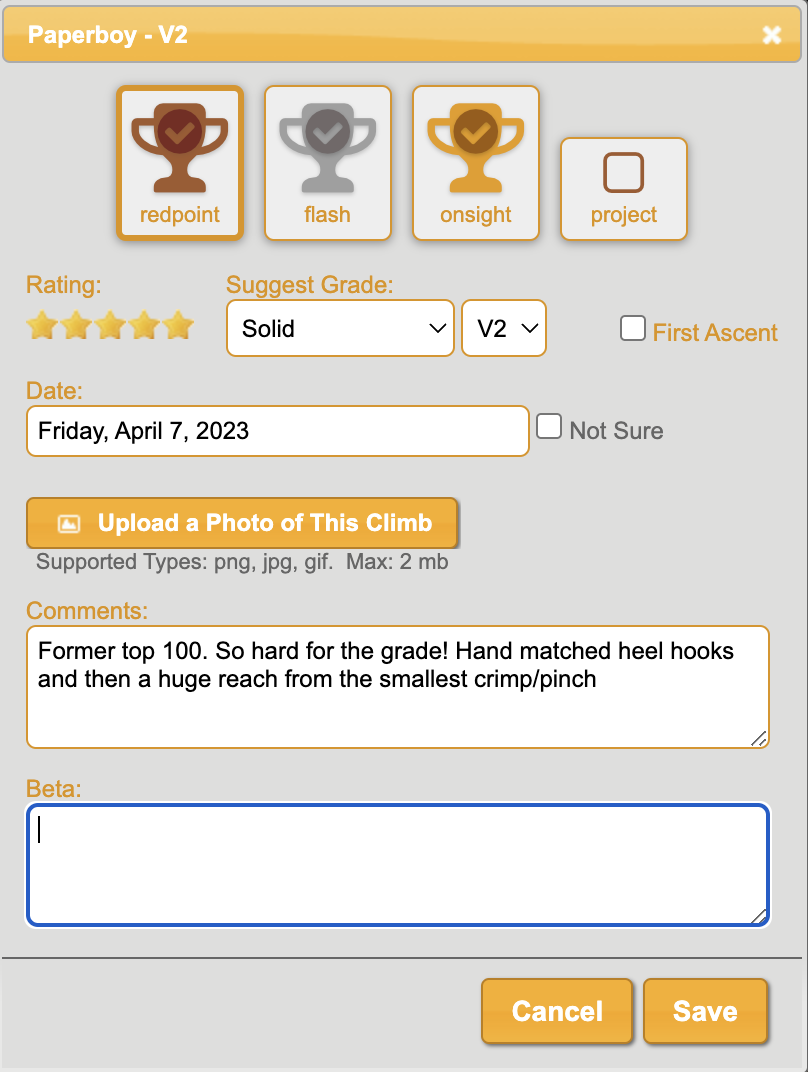
\includegraphics[scale=0.4]{sendage.png}
  \caption{For each send, the boulderer logs the date, any comments and/or "beta" used (the holds, moves or sequence to climb the boulder); they can rate the problem 1-5 stars and give a "feels-like" grade. The date defaults to the current date, so we can expect a few days error in some logged climbs if users do not manually set the actual date the problem was climbed. The default grade is the mean grade of previous logged sends; this biases the user heavily to agree to already proposed grades.}
  \label{fig:sendage}
\end{figure}


\section{Data}

All models were trained on data from the climbing website \href{https://sendage.com}{sendage.com} created and maintained by Jamie Chong, a developer and climber based in Vancouver. It's similar to the larger more well known site 8a.nu, but the climb information is far more heavily currated creating a much cleaner dataset with accurate location data for climbs and practically no duplicates. 

I limited my analysis to boulders, as opposed to sport climbs and trad climbs, because they are more heavily tracked on the site. The most popular boulder problem, Superfly, has nearly 700 "sends" vs 240 ascents of the most popular sport route, Rug Munchers; 45 boulders have more logged sends than Rug Munchers. The most popular trad route, Diedre, has only been logged 186 times, despite there being a queue of parties waiting for Diedre when the weather clears. 

To ensure enough data for boulder problems and boulderers alike, I filtered down to a self consistent set of problems with at least 5 sends and boulderers that sent at least 5 boulders. For BC, that reduces to 2844 boulder problems, 1069 boulderers that logged 68,336 sends; if I include much of the world, that only increases to 5367 problems, 1428 boulderers with 116,997 sends (the site is mostly used by BC climbers). 


Figure \ref{fig:sendage} shows a sendage window to log a climb. The mean rating is -- with -- fraction rated; -- / -- / -- fraction have a date, comments or beta, respectively. The mean range of assigned grades to a particular problem is less than 1 V grade; the maximum range is 2 V grades\footnote[1]{\href{https://www.99boulders.com/bouldering-grades}{Bouldering grades} in North America follow the "V scale" that was created by John Sherman in the 1980s. A beginner shouldn't be surprised if even V0 feels impossible; there are currently four boulders with the proposed grade V17 and only one of these has seen repeats to confirm the grade.}. The most popular grade logged is V4 with a linear drop up to V11 and a few harder sends up to V14; likewise, there are fewer V0-V3 boulders logged: many climbers don't log the "easy" problems. 



Likely to be very detailed if the datasets are new or unfamiliar to the community, or if familiar datasets are being used in new ways.
Includes prior work on them, statistics, and a collection protocol. 

\section{Model}

Flesh out your own approach, perhaps amplifying themes from the `Prior lit' section.

\section{Methods}

The experimental approach, including descriptions of metrics, baseline models, etc. Details about hyperparameters, optimization choices, etc., are probably best given in appendices, unless they are central to the arguments.

Explicitly define the metrics, even the common ones (or at least reference them). Be clear about how the data is split for assessment. 

\section{Results} 

A no-nonsense report of what happened.

\section{Analysis} 

Discussion of what the results mean, what they don’t mean, where they can be improved, etc. These sections vary a lot depending on the nature of the paper. (For papers reporting on experiments with multiple datasets, it can be good to repeats Methods/Results/Analysis in separate (sub)sections for each dataset.)

\section{Conclusion} 

Quickly summarize what the paper did, and then chart out possible future directions that anyone might pursue.

\section*{Known Project Limitations}

For this section, imagine that your reader is a well-intentioned NLP practitioner who is seeking to make use of your data, models, or findings as part of a separate scholarly project, deployed system, or some other kind of real-world intervention. What should such a person know about your work? Especially important here are limitations and biases that might affect this person, their findings, their experiment participants, or the users of their product or service. The idea is that what you say here will be taken into consideration but this well-intentioned user, leading to better outcomes for everyone.

\section*{Authorship Statement}

I worked on this project solo including the literature review, the iterative implementation and experimentation, result gathering and final writing up. I had many fruitful conversations with Alistair Fraser, also taking the course, and Michael Nathe about my design choices and result analysis. 

\bibliography{project}

% \appendix

% \section{Example Appendix}\label{sec:appendix}

% This is an appendix.

\end{document}
